\chapter{Dynamic Robot Swarm Networks}
\label{chapter5}
	% This is the third use-case for EMANE
		% Combinatation use-case:
			% Work with other software
			% Emulate a distributed, dynamic network
This chapter presents the third and final use case for EMANE that was explored in this thesis.
The primary work that will be covered relates to extending the robot swarm simulator ARGoS~\cite{argos}, to introduce emulated communication models.
	% Overview of the swarm + swarm network architecture
		% Swarm of 25 robots deployed to make environmental observations
		% Example deployment to wildfire (hostile area, remote)		
	% Use wireless comm links to share information with each other to:
		% Maintain the network
		% Share information between robots (to make better decisions)
		% Return information back to central command
The network outlined in this chapter consists of a swarm of 25 simulated flying robots that are tasked with identifying wildfire in an area.
By operating in the context of a wildfire, several environmental factors are introduced that must be considered.
Primarily, the conditions this network is present in are not prime for wireless communications as smoke or other obstacles may exist, and well-deployed, centralized infrastructure is unlikely to be present.
To this end, communications must happen in a distributed manner across the swarm mesh, and traffic must be relayed to reach a command center.
	% This network is a MANET (EMANE's specialty)
		% Routing is key (the links connect and disconnect rapidly)
These conditions are the ideal operating parameters for a mobile ad-hoc network (MANET) configuration, which is EMANE's specialty.
By using EMANE and ARGoS together, this unique network behavior can be appropriately captured.

\section{Extending Existing Software}
    % Introduce ARGoS
    		% A  robot swarm simulator  
        % ARGoS models the behavior of robots in the network and the environment they operate in
			% How they move
			% What data they need to be transferred
				% Based on operating algorithms
        % ARGoS operates in chunks of time instead of real, continuous time like EMANE
        		% Configurable, but for the purpose here ARGoS simulates 100ms at a time
        		% Important to understand the time-scale differences
        			% Will impact integration methodologies
The robot swarm simulator, ARGoS, is a physics based simulator designed with the intent filling the gap for large-scale heterogeneous robot swarms~\cite{argos}.
The tool models the swarm and controls the environment it operates in, modeling the movement, physics, and information transfer of the individual robots.
One of the key attributes about ARGoS that is essential to understand, is the manner in which ARGoS performs its simulation.
ARGoS will simulate the functionality of the swarm in specified time chunks.
This is different from EMANE which operates in real-time, and needing to account for these fundamental differences influences the design process of integration.
	% Why integrate EMANE with ARGoS?
		% Introduce more accurate communication modeling
			% ARGoS can perform basic communication modeling
				% One example of implementation is check for line of sight conditions
				% No measure of channel effects
					% Pathloss, TX/RX Power level
					% Packet corruption, delay, duplication
					% Latency
					% Throughput   		
		% Can use the full implementation of B.A.T.M.A.N. or other routing/networking software
			% Instead of coding the behavior of B.A.T.M.A.N. (or other routing from scratch) and having to verify it is functionally the same, use EMANE to run actual B.A.T.M.A.N.
				% The behavior can't be different if the program is the exact same as would be used in hardware
		% Introduce machine learning to influence routing software
            % Machine learning models can run in real time in each EMANE node, and can communicate with other models and nodes through the EMANE network
            % Allows the same models to run in EMANE as would run on the physical robot
There are several reasons why it is beneficial to integrate the two tools.
For one, EMANE on its own does not handle the mobility of nodes, the traffic that travels the network, or the management of an environment.
These are all things that must be set up externally, and as such having ARGoS handle them is a natural fit.
In the other direction, having EMANE handle communication for ARGoS can allow more accurate modeling of channel effects.
ARGoS has basic ``medium'' plugins (the type of plugin responsible for communications), but these can be rather simple.
One such model, simply determines if two robots are within a set range, and have line of sight (LOS).
If these conditions are true then the two robots are free to exchange information with no delay or maximum datarate.
Another benefit to using EMANE is the ability to use the native implementation of the B.A.T.M.A.N. routing protocol.
By deploying this protocol on EMANE, it can be further tested and developed in a proper swarm environment.

\section{Integrating the Software}
This section will detail the integration of EMANE and ARGoS and how the two software operated together.
The following section will shed light on several of the design decisions that were made and explain the rationale behind them.\par
    % Two simulation/emulation programs run simultaneous on the same machines
        % ARGoS and EMANE are both configured and run separately
            % They exist as separate processes during the extent of runtime (one is not a child of the other) 
	% A third process exists (EMANE Interface Manager)
		% EMANE on its own is a collection of programs
		% Requires something to manage all of the processes
		% Python script that runs as the broker between ARGOs and EMANE proper
ARGoS and EMANE both ran on the same machine for the purposes of their integration.
EMANE also had an additional program that acted as an intermediary between it and ARGoS, as EMANE is not a single process and needed something to manage it.
Each process was also completely separate from the other, neither process was a child.
This is important to understand as it dictated how the two processes attached to each other.
If one process was a child of the other, they would naturally be connected. Instead, part of the initialization processing was the two processes connecting.
    % ARGoS starts by opening shared memory and populates with metadata (including process ID) during it's initialization phase
		% (Table: Shared Memory Metadata)
  		% By providing PIDs, the two programs can interact with each other
ARGoS began the process by opening a shared memory location with a name known by both ARGoS and EMANE.
This shared memory contained metadata pertaining to the simulation including the process ID (PID) of ARGoS, the number of robots in the experiment, and the timescale being used.
Table~\ref{shm_meta} details the exact content of the shared metadata.
\begin{table}[!ht]
\centering
\caption{Contents of the shared memory metadata file. Includes which processes are responsible for what data}
\begin{adjustbox}{width=0.8\textwidth, center=\textwidth}
	\begin{tabular}{l|c|l}
		\multicolumn{1}{c|}{Provided By} & Type & Data \\ 
		\hline
		ARGoS & uint16\_t & Number of Robots \\
		ARGoS & uint16\_t & Number of Communication Robots \\
		ARGoS & double & ARGoS Timescale \\
		ARGoS & pid\_t & ARGoS Process ID \\
		EMANE & pid\_t & EMANE Process ID
	\end{tabular}
\end{adjustbox}
\label{shm_meta}
\end{table}
	% ARGoS then goes to sleep after initialization, waiting for EMANE-Interface to find the shared memory, and do its setup
		% Since the location of the shared memory is known, one of the processes (the one that doesn't make it) can find information from the other without knowing the PID of the other
	% EMANE-Interface populates the rest of the metadata (primarily just its PID) and sets up a shared memory location for robot pose information (location data), and robot communication data (amount of data requested to be transferred)
		% (Table: Shared Memory Pose)
		% (Table: Shared Memory Comm)
		% ARGoS knows where to find these shared memories (ARGoS does not create them itself because originally EMANE was supposed to create all of them, this led to issues with step 1)
		% EMANE-Interface then sets up internal data structures to store robot information and communication before waking ARGoS and going to sleep
After populating this data, ARGoS put itself to sleep and waited for EMANE to indicate it was ready.\par
EMANE started up during this time and waited until it could find the shared memory structure and to get ARGOS's PID.
With this PID, EMANE was able to directly communicate with ARGoS.
EMANE then set up the remaining two shared memory locations, and set up its internal data structures.
The second shared memory structure was used by ARGoS to deliver information about the location and pose of robots to EMANE.
This was essential for ensuring both programs had the same representation of the virtual environment.
Table~\ref{shm_pose} outlines the exact contents of this memory block.
\begin{table}[!ht]
\centering
\caption{Contents of the shared memory robot pose file. Includes which processes are responsible for what data}
\begin{adjustbox}{width=0.6\textwidth, center=\textwidth}
	\begin{tabular}{l|c|l}
		\multicolumn{1}{c|}{Provided By} & Type & Data \\ 
		\hline
		ARGoS & uint16\_t & Robot ID \\
		ARGoS & double\_t & Robot Latitude \\
		ARGoS & double & Robot Longitude \\
		ARGoS & double & Robot Altitude
	\end{tabular}
\end{adjustbox}
\label{shm_pose}
\end{table}
The third shared memory structure was used by both ARGoS and EMANE to deliver relevant data to performing communications.
ARGoS used the block to make requests of EMANE and EMANE used it to response with the requested information.
Table~\ref{shm_comms} outlines the exact contents of this memory block.\par
\begin{table}[!ht]
\centering
\caption{Contents of the shared memory robot communications file. Includes which processes are responsible for what data}
\begin{adjustbox}{width=0.7\textwidth, center=\textwidth}
	\begin{tabular}{l|c|l}
		\multicolumn{1}{c|}{Provided By} & Type & Data \\ 
		\hline
		ARGoS & uint16\_t & Transmitting Robot ID \\
		ARGoS & uint16\_t & Receiving Robot ID \\
		ARGOS & uint8\_t\* & Message Pointer \\
		ARGoS & uint32\_t & Message Size \\
		EMANE & uint32\_t & Amount of data transmitted
	\end{tabular}
\end{adjustbox}
\label{shm_comms}
\end{table}
Having set up all the relevant structures used to communicate, the processes were ready to proceed with actual simulation.
This began when EMANE woke up ARGoS for the first time.
The two processes controlled each other via POSIX signals, specifically the \textit{SIGSTOP} and \textit{SIGCONT} signals.
These signals indicated to the operating system if a process should be put to sleep or woken from sleep.
When a process was done with its turn, it signaled the other with a \textit{SIGCONT} and then raised its own \textit{SIGSTOP} to indicate to the operating system to put it should be put to sleep.
	% The two processes communicate with each other using POSIX signals, specifically SIGSTOP to put itself to sleep and SIGCONT to wake itself
		% These signals are nice because the OS will handle stoping and waking the processes, and as such the singals are caught and handled before arriving at the process
The main loop then began between the programs.
	% ARGoS takes its turn, moving robots, sensing the environment, etc. for 100ms before it updates information about the robot poses, and communication pairs
ARGoS first took its turn, moving robots, sensing the environment, and making determinations about information sharing for 100ms of simulation time.
Once it finished the period, it updated the relevant information across the shared memory segments and initiated EMANE.
	% EMANE-Interface then takes its turn, simulating 100ms of communication, updates shared data, and starts ARGoS
		% This is done using a simple throughput test (iperf) to determine how much data can travel through the network to a give node
		% Because there is no way to measure 100ms of data transfer easily, EMANE-Interface extrapolates the amount of data sent by dividing the speed over 1 second by 10
	% This continues until ARGoS is finished with its experiment, at which point ARGoS starts a new experiment or terminates, informing EMANE-Interface of termination
The EMANE interface script woke up and updated its internal store of information.
Any new location data was sent into the emulator via location events so that the corresponding NEMs would move into the appropriate location and update their communication links.
EMANE then began the process of emulating communications.
This was done by measuring the throughput to adjacent nodes, instead of performing actual data transfers. The reasoning for this is explained in the following section.\par
Once EMANE collected all the required information from its throughput tests, it populated that information back into the shared memory blocks and woke ARGoS, starting the process over again.
This then continued until ARGoS finished its current experiment, at which point it either reset, or terminated.
In the case of termination, ARGoS signals EMANE to also shutdown.
If ARGoS is immediately starting another experiment, EMANE is not informed as the transition between experiments is entirely transparent to EMANE.
Figure~\ref{emane_argos} shows the layout of all the pieces of software required to connect EMANE and ARGoS.
Appendix~\ref{appendixc} contains the full source code of the EMANE side of the integration process.
\begin{figure}[!ht]
    \centering
    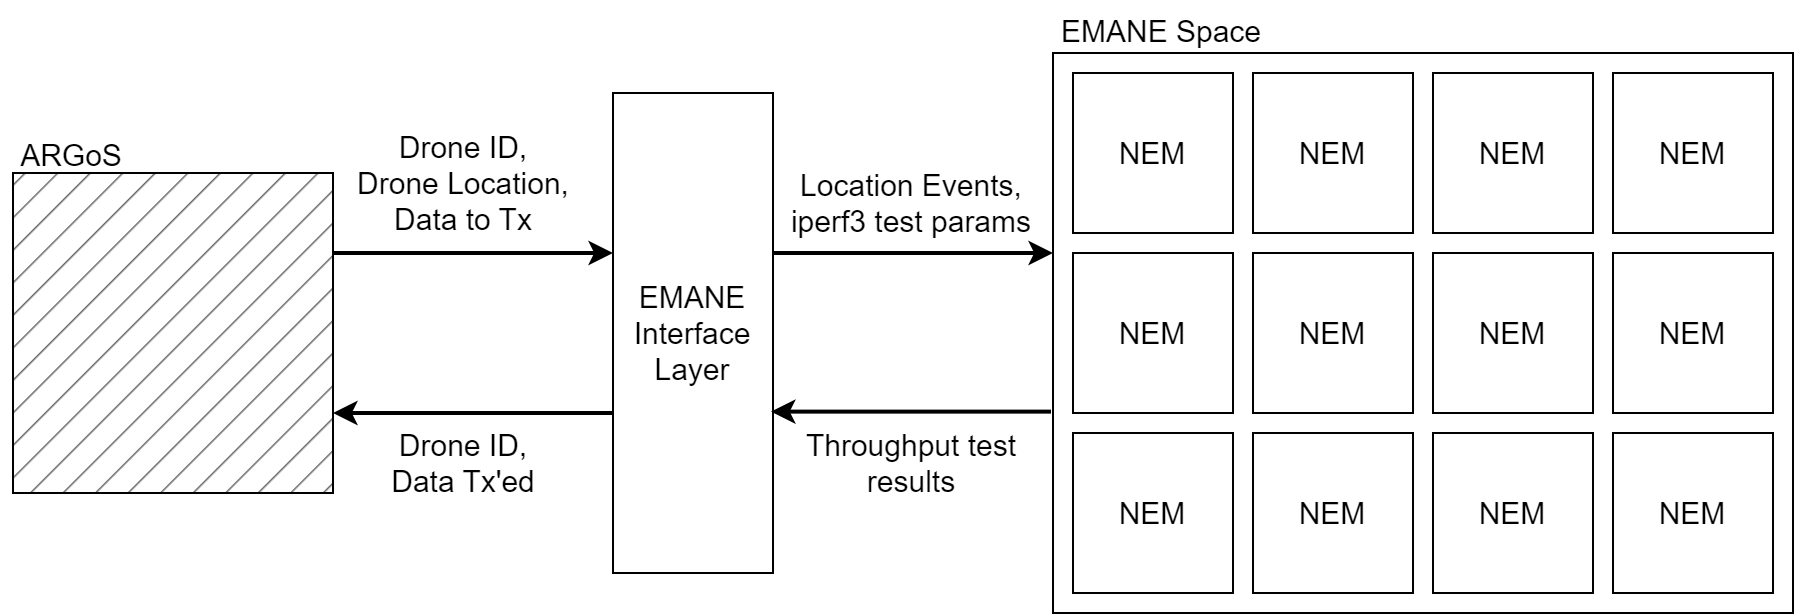
\includegraphics[width=\textwidth,keepaspectratio]{Images/Chpt5/ARGoS-EMANE.png}
    \caption{The topology of the ARGoS-EMANE integration system. All the major systems as well as the interconnections between them are displayed.}
    \label{emane_argos}
\end{figure}

\section{Integration Design Decisions}
	% Several desisions during the design of the above proces had to be made
		% These decisions were made in the hopes to maximize performance, minimize latency, and ensure stability
Several design decisions were made during the development of the above process with the goal of maximizing the performance of the interface, minimizing the latency between each process running, and ensuring the system remained stable.
The two biggest decisions made were the decision to use shared memory for information sharing and the decision to abstract the data being sent through EMANE.
These decisions ensured that the interface would still be accurate, without introducing unnecessary complexities that would further slow down the system.\par 
    % Why were certain design decisions made?
        % Shared memory
            % Less latency than something like a socket
            % The amount and size of data is known enough that appropriate blocks of memory can be opened
It was decided that one or more shared memory segments should be used to pass information between processes.
Transferring data over the network was deemed needlessly slow and complex.
The time taken to output data from the tool, package it appropriately, send it over the network, unpack it, and import it would have a taken an order of time longer than the actual time needed to generate and consume the data being sent.
Since networking was not to be used, both processes needed to run on the same machine and have access to the same hardware.
For the same reason that using networking would be too slow, performing file I/O to read and write data to a file would have also been too slow.
Since both processes are capable of accessing memory incredibly quick, using the operating system to grant ARGoS and EMANE access to the same location in system memory was the logical solution.\par
The second major design decision, was to not provide EMANE with the exact data payloads ARGoS was sending between robots.
    % Why abstract transmission -> (Don't send actual payload through EMANE)
        % Sending the actual payload would require lots of additional work (each robot in ARGoS would need to deliver its payload to its corresponding node in EMANE, and then retrieve any data waiting for it)
        % The payoff from this work was deemed not worth it as the behavior of informing each robot how much data it sent and received accomplished the same goal
        % The payload was not being sent with a lossless protocol so the behavior of if the data arrives or not is much more important (robots would not be retransmitting)
ARGoS, and the algorithm running on the robots, was not concerned with any form of transmission control or retransmission upon failed delivery of data.
This means that EMANE did not need to worry about what data successfully made it to the receiver, just how much of it arrived.
By avoiding handing off the entire data payload to EMANE, time could be saved and a layer of complexity was removed.
EMANE instead can just characterize the transmission, and inform ARGoS on what amounts of data can be given to each robot in a certain timeframe.
This does not compromise the validity of the channel effects EMANE imparts on transmission, as throughput and latency were the primary two metrics being modeled anyway (as observed in Chapter~\ref{chapter3}).\par
	% Issues with C vs Python programming languages (typing and shared memory)
One of the major issues during development that had to be addressed was the difference in programming languages used.
ARGoS, and therefore its portion of the interface code, was written in C++.
The EMANE interface manager, was written in Python.
Since data was being accessed directly from memory, it was important that the exact size of the data was accurately read.
C++ provides the user with data types that are not present in Python, with most data types in Python taking up larger amounts of space than the closest equivalent in C/C++.
Even when using a library such as \textit{ctypes}, meant to introduce more ``C-like'' types, the problem was still present.
The solution ended up being to serialize and deserialize the data instead of mapping the memory directly to a structure, as was done in C++.
The following code snippet uses a format string to interpret the exact number of bytes each variable should be for serialization and serialization:
\begin{minted}[fontsize=\footnotesize, breaklines]{python}
__struct_format: str = 'HHdIIddd'

def unpack(self, shm):
	self.num_drone, self.num_comms, self.deltaT, self.argos_pid, self.emane_pid, self.gw_lat, self.gw_lon, self.gw_alt \
		= struct.unpack(self.__struct_format, shm.buf.tobytes())
\end{minted}
This solution worked well to solve the problem, and while it may have been slower than the process used for memory access in C++, it was still much faster than EMANE takes and did not affect overall run time.
Further testing can be performed to determine if the interface script would have an improvement on performance if written entire in C++.

\section{Integration Results}
	% EMANE and ARGoS are capable of working together
		% Demonstrate ARGoS moving EMANE nodes
The basic ability for ARGoS and EMANE to pass information back and forth is presented, with ARGoS delivering robot locations and EMANE delivering communications metrics, but several factors remain to be implemented or improved upon.
Figure~\ref{emane_locs} shows a printout of EMANE's event channel.
By using the \textit{emaneevent-dump} utility, any events sent through EMANE can be observed.
As observed in Figure~\ref{emane_locs}, EMANE received location events over time as ARGoS updated the manager script with new locations.
\begin{figure}[!ht]
    \centering
    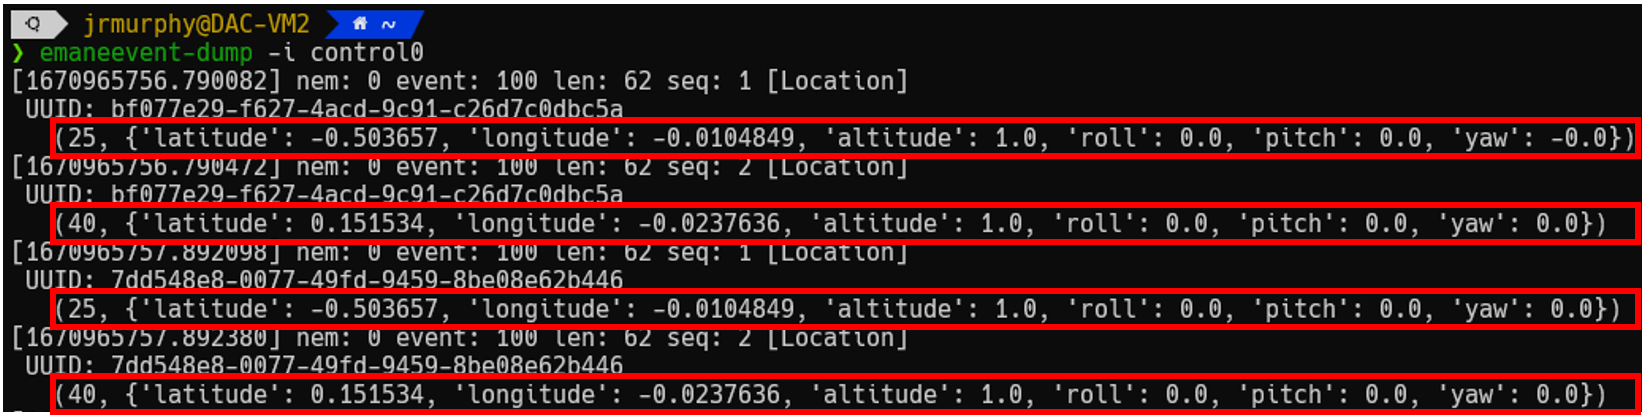
\includegraphics[width=0.85\textwidth,keepaspectratio]{Images/Chpt5/ARGoS_Events_EMANE_annotated.png}
    \caption{A dump of several events that were sent over the EMANE event channel. These location events show that ARGoS is delivering location data to the interface script, which is subsequently delivering location events to EMANE.}
    \label{emane_locs}
\end{figure}
It can be seen from the initial numbers in square brackets that these events were only firing about every one second.
Since these events should be firing for every 100ms of simulation time, we see that simulating 100ms of time took ARGoS and EMANE a combined ten times longer.
This behavior was expected from the start, but the extent of how bad it would be had been unknown.\par
EMANE runs in real-time and therefore at a minimum would take 100ms to create 100ms of data.
However, because the network needs time to reconfigure after locations are updated, and the throughput tests need time to record data, it is much more likely that EMANE takes anywhere from two to five times as long to generate that data.
The extended run-time above is on the extreme side and was recorded before optimizations were started, but additional optimizations would be needed to bring that number down further, if possible.
As a final point to understand the extent of the slowdown imparted on ARGoS by combining it with a real-time emulator, ARGoS running in isolation using an internal communication medium plugin only takes about four seconds to run a 10-minute experiment.
With the best case scenario of EMANE adding 200ms of time per 100ms emulation block, the ten-minute experiment would now take twenty minutes.
This length of emulation may be an acceptable trade off for the features EMANE brings to the testbed, but is an essential consideration that must be made.
	% However, EMANE seriously slows down ARGoS
		% We expected this
		% EMANE is an emulator and runs at a minimum, real time
		% What are the performance differences between ARGoS Standalone and ARGoS + EMANE
			% ARGoS Standalone takes 4 seconds for a 10 minute experiment
			% ARGoS+EMANE takes 20min or more for the same experiment (with most basic settings)
				% Not including any checking of latency, just pure data return
		% Can we make it faster?

\section{Chapter Summary}
This chapter focused on introducing additional tools to EMANE to enable EMANE to more dynamically model certain networks.
By interfacing with the ARGoS robot simulation tool, both tools receive enhancements in the forms of more accurate modeling of all parts of a robot swarm network.
The primary results found were that the software are able to communicate through the designed methodology, but the real-time nature of EMANE slows down ARGoS drastically.
At the time of writing the interface is in the earlier stages of development with only the basic functionality presented here implemented.
The work is being continued to further optimize the process and deliver additional functionality.
